\chapter{Entropy and Free Energy of Reaction}\label{ch:b2:reaction-free-energy}

A sports cold pack holds a bag of water and a few spoonfuls of ammonium
nitrate. Squeeze it, the inner bag bursts, the salt dissolves, and within
seconds the pack is cold enough to soothe a sprained ankle. The dissolution
absorbs heat --- it is \omterm{def:b2:reaction-enthalpy:exothermic}{endothermic} --- and yet it runs on its own, to
completion. The enthalpy of the previous chapter cannot be the whole story:
a reaction does not go only ``downhill in heat''. The missing quantity is
entropy, which the second law of thermodynamics, met in physics, makes the
judge of every spontaneous change. This chapter tabulates entropies,
computes the entropy of a reaction, and combines enthalpy and entropy into
one function, the \omterm{def:b2:reaction-free-energy:gibbs-energy}{Gibbs energy}, whose reaction derivative decides the
direction of every reaction at fixed temperature and pressure.

\begin{recall}
From physics: the second law. Every system has a state function, its
entropy $S$ (extensive); in a transformation of a closed system, $\dd S =
\delta Q/T_{\text{ext}} + \delta S_{\text{c}}$, where the created entropy
$\delta S_{\text{c}}$ is zero for a reversible change and positive
otherwise; for a closed system of fixed composition, $\dd U = T\dd S -
p\dd V$. \Cref{ch:b2:reaction-enthalpy}: reaction quantities $\Delta_r X =
(\partial X/\partial\xi)_{T,p}$ and standard reaction enthalpies. The Year 1
volume stated, as laws ``that follow from the second law'', that a
reaction evolves until $Q = K^\circ$; this chapter and the next two derive
them.
\end{recall}

\begin{omfigure}
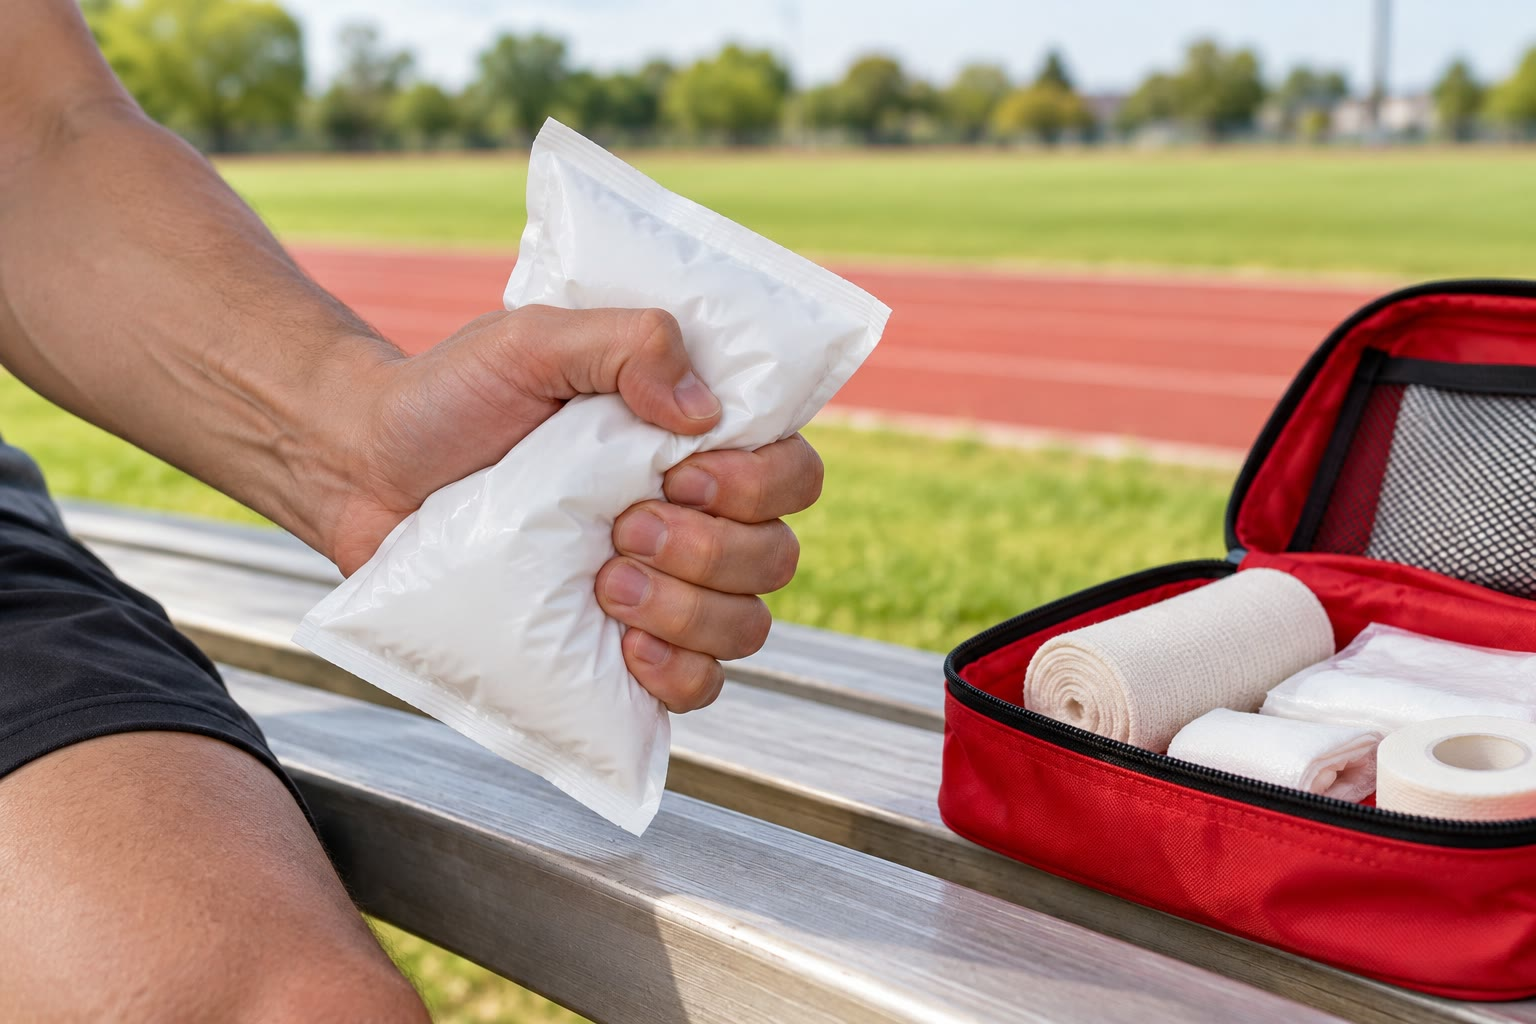
\includegraphics[width=0.55\linewidth]{images/book3/ai/b2-02-cold-pack.jpg}

{\small A cold pack: when its inner bag is broken, ammonium nitrate
dissolves in water and the pack cools. The dissolution is \omterm{def:b2:reaction-enthalpy:exothermic}{endothermic} and
spontaneous; its entropy explains why (\cref{ex:b2:reaction-free-energy:cold-pack}).}
\end{omfigure}

\section{Standard entropies and the third law}

Unlike enthalpy, entropy has a natural zero.

\begin{theorem}[Third law of thermodynamics]\label{thm:b2:reaction-free-energy:third-law}
The entropy of a pure, perfectly ordered crystal tends to zero as its
temperature tends to \qty{0}{K}.
\end{theorem}
\admitted

\begin{remark}[Where the zero comes from]\label{rem:b2:reaction-free-energy:third-law}
Walther Nernst stated in 1906 that reaction entropies between condensed
phases vanish as $T \to 0$; Max Planck sharpened it into the statement
above. Its origin is statistical: entropy counts the microscopic
arrangements compatible with the state of a system, and a perfect crystal
at \qty{0}{K} has a single one. The counting is done in the Year 3 volume,
with partition functions.
\end{remark}

\begin{definition}[Standard molar entropy]\label{def:b2:reaction-free-energy:standard-entropy}
The \emph{standard molar entropy}\index{standard molar entropy}
$S^\circ_m(T)$ of a substance is the entropy of one mole of it in its
standard state at temperature $T$, the zero being that of the third law.
Unlike $\Delta_f H^\circ$, it is an absolute quantity, positive for every
substance, elements included.
\end{definition}

\begin{proposition}[Absolute entropy from heat capacities]\label{prop:b2:reaction-free-energy:absolute-entropy}
Heating a substance at constant pressure $p^\circ$ from \qty{0}{K} to $T$,
\[
  S^\circ_m(T) = \int_0^T\frac{C^\circ_{p,m}(T')}{T'}\,\dd T' +
  \sum_{\text{transitions}}\frac{\Delta_{\text{trs}}H^\circ}{T_{\text{trs}}} ,
\]
the integral being taken in each phase over its range of temperature.
\end{proposition}

\begin{proof}
Heat the substance reversibly at constant pressure: $\delta S_{\text{c}} =
0$ and $\delta Q = \dd H = C_p\,\dd T$, so $\dd S = C_p\,\dd T/T$. At a
transition (melting, boiling) the temperature stays at $T_{\text{trs}}$
while the heat $\Delta_{\text{trs}}H$ is received reversibly: the entropy
jumps by $\Delta_{\text{trs}}H/T_{\text{trs}}$. Add the pieces from the
third-law zero.
\end{proof}

\begin{omfigure}
\begin{tikzpicture}
\begin{axis}[
  width=0.8\linewidth, height=6.2cm, xmin=0, xmax=1500, ymin=0, ymax=210,
  axis x line=bottom, axis y line=left, xlabel={$T$ (K)},
  ylabel={$S^\circ_m$ of zinc (\unit{J/(K.mol)})},
  xtick={0,250,500,750,1000,1250,1500},
  tick label style={font=\small}, label style={font=\small}, clip=false]
\addplot[omDef, very thick, smooth] table[x=T, y=S] {figdata/out/bachelor-2-standard-entropy-solid.dat};
\addplot[omProp, very thick] table[x=T, y=S] {figdata/out/bachelor-2-standard-entropy-liquid.dat};
\addplot[omThm, very thick] table[x=T, y=S] {figdata/out/bachelor-2-standard-entropy-gas.dat};
\draw[densely dashed, gray] (axis cs:692.73,64.6) -- (axis cs:692.73,75.2);
\draw[densely dashed, gray] (axis cs:1180.2,91.9) -- (axis cs:1180.2,189.6);
\node[omDef, font=\small, anchor=south east] at (axis cs:600,60) {solid};
\node[omProp, font=\small, anchor=north west] at (axis cs:850,78) {liquid};
\node[omThm, font=\small, anchor=south] at (axis cs:1350,192) {gas};
\node[font=\scriptsize, anchor=west, align=left] at (axis cs:700,110) {melting, $+10.6$\\ at \qty{692.7}{K}};
\node[font=\scriptsize, anchor=east, align=right] at (axis cs:1170,150) {boiling,\\ $+97.7$ at\\ \qty{1180.2}{K}};
\end{axis}
\end{tikzpicture}

{\small \omterm{def:b2:reaction-free-energy:standard-entropy}{Standard molar entropy} of zinc from the third-law zero. It grows
with temperature as the metal stores heat, then jumps at the melting point
by $\Delta_{\text{fus}}H/T_{\text{fus}}$ and, much more, at the boiling
point by $\Delta_{\text{vap}}H/T_b$: a gas is far more disordered than a
liquid.}
% ledger: s0T:Zn_crl.0, s0T:Zn_crl.298.15, s0T:Zn_cr.692, s0T:Zn_l.692, s0T:Zn_l.1180, s0T:Zn_g.1180, hT:Zn_cr.692, hT:Zn_l.692, hT:Zn_l.1180, hT:Zn_g.1180, dfh:Zn_g (curve in figdata/bachelor-2/standard-entropy.py)
\end{omfigure}

The figure gives orders of magnitude worth remembering. At room
temperature a metal or a hard crystal holds a few tens of
\unit{J/(K.mol)}, a liquid around a hundred, a gas one to three hundred;
melting adds a little, boiling adds a lot. The standard molar entropies
used in this volume are tabulated with the formation enthalpies.

\section{Reaction entropy}

\begin{definition}[Reaction entropy]\label{def:b2:reaction-free-energy:reaction-entropy}
The \emph{reaction entropy}\index{reaction entropy} is $\Delta_r S =
(\partial S/\partial\xi)_{T,p}$, and the \emph{standard reaction
entropy}\index{standard reaction entropy} is $\Delta_r S^\circ(T) =
\sum_i\nu_iS^\circ_{m,i}(T)$, in \unit{J/(K.mol)}.
\end{definition}

Because standard entropies are absolute, no formation reaction is needed:
the elements count with their own entropies.

\begin{example}[Three reaction entropies]\label{ex:b2:reaction-free-energy:entropies}
At \qty{298.15}{K}:
\begin{itemize}
  \item \ce{CaCO3(s) -> CaO(s) + CO2(g)}: $\Delta_r S^\circ = 39.75 + 213.79 -
        92.9 = \qty{+160.6}{J/(K.mol)}$, a gas made from a solid;
  \item \ce{N2(g) + 3H2(g) -> 2NH3(g)}: $\Delta_r S^\circ = 2(192.77) -
        191.61 - 3(130.68) = \qty{-198.1}{J/(K.mol)}$, four molecules of gas
        becoming two;
  \item \ce{N2O4(g) -> 2NO2(g)}: $\Delta_r S^\circ = 2(240.03) - 304.38 =
        \qty{+175.7}{J/(K.mol)}$.
\end{itemize}
% ledger: s0:CaCO3_cr, s0:CaO_cr, s0:CO2_g, s0:N2_g, s0:H2_g, s0:NH3_g, s0:N2O4_g, s0:NO2_g (computed in figdata/bachelor-2/thermo-data.py)
\end{example}

\begin{proposition}[The sign of a reaction entropy]\label{prop:b2:reaction-free-energy:sign-rule}
When gases take part, the sign of $\Delta_r S^\circ$ is in general that of
$\Delta\nu_{\text{gas}} = \sum_{\text{gases}}\nu_i$, and its size is about
\qty{100}{} to \qty{200}{J/(K.mol)} per mole of gas made or consumed. When
$\Delta\nu_{\text{gas}} = 0$, or no gas is involved, $\Delta_r S^\circ$ is
small and its sign must be computed.
\end{proposition}

\begin{proof}[Justification]
The molar entropy of a gas at \qty{298}{K} is between 130 and
\qty{300}{J/(K.mol)}, that of a solid or a liquid a few tens: making or
consuming one mole of gas dominates every other contribution. This is a
rule of thumb, not a theorem: the dissolution of a salt, with no gas, can
still change the entropy by a hundred \unit{J/(K.mol)}.
\end{proof}

\begin{method}[Predicting the sign of $\Delta_r S^\circ$]\label{met:b2:reaction-free-energy:entropy-sign}
\begin{enumerate}
  \item Count $\Delta\nu_{\text{gas}}$: if it is not zero, it gives the
        sign.
  \item Otherwise compare the order of the states: dissolving a crystal,
        melting, breaking a molecule into two pieces raise the entropy;
        precipitating, freezing, joining two molecules into one lower it.
  \item When the decision matters, compute $\sum_i\nu_iS^\circ_{m,i}$.
\end{enumerate}
\end{method}

The Year 1 volume met a consequence: an elimination makes more molecules
than a substitution with the same reagents (the alkene, the leaving group
and the protonated base, against the substitution product and the leaving
group). Its \omterm{def:b2:reaction-free-energy:reaction-entropy}{reaction entropy} is larger, and the entropy term, which grows
with temperature as shown in the next section, is why heat favours
elimination over substitution.

\section{The Gibbs energy}

\begin{definition}[Gibbs energy]\label{def:b2:reaction-free-energy:gibbs-energy}
The \emph{Gibbs energy}\index{Gibbs energy} (or free enthalpy) of a system
is the state function $G = H - TS$, extensive, in joules.
\end{definition}

\begin{definition}[Reaction Gibbs energy]\label{def:b2:reaction-free-energy:reaction-gibbs}
The \emph{reaction Gibbs energy}\index{reaction Gibbs energy} is $\Delta_r G
= (\partial G/\partial\xi)_{T,p}$, and the \emph{standard reaction Gibbs
energy}\index{standard reaction Gibbs energy} is $\Delta_r G^\circ(T) =
\sum_i\nu_iG^\circ_{m,i}(T)$, both in \unit{kJ/mol}.
\end{definition}

\begin{proposition}[Enthalpy and entropy terms]\label{prop:b2:reaction-free-energy:g-h-s}
$\Delta_r G = \Delta_r H - T\Delta_r S$, and $\Delta_r G^\circ = \Delta_r
H^\circ - T\Delta_r S^\circ$.
\end{proposition}

\begin{proof}
Differentiate $G = H - TS$ with respect to $\xi$ at fixed $T$ and $p$: $T$
is a constant of the derivative.
\end{proof}

\begin{proposition}[Differential of $G$ for a reacting system]\label{prop:b2:reaction-free-energy:dG}
For a closed system in which one reaction takes place, at uniform $T$ and
$p$,
\[
  \dd G = V\,\dd p - S\,\dd T + \Delta_r G\,\dd\xi .
\]
\end{proposition}

\begin{proof}
$G(T, p, \xi)$ has the exact differential $\dd G = (\partial G/\partial
T)_{p,\xi}\dd T + (\partial G/\partial p)_{T,\xi}\dd p + \Delta_r G\,\dd\xi$.
The first two partial derivatives are taken at fixed composition: they are
those of a closed system of fixed composition, for which physics gives
$\dd U = T\dd S - p\dd V$, so that $\dd G = \dd U + p\dd V + V\dd p - T\dd S
- S\dd T = V\dd p - S\dd T$. Hence $(\partial G/\partial T)_{p,\xi} = -S$
and $(\partial G/\partial p)_{T,\xi} = V$.
\end{proof}

\section{The evolution criterion}

\begin{theorem}[Evolution criterion]\label{thm:b2:reaction-free-energy:evolution}
In a closed system kept at constant temperature and pressure, exchanging no
work other than that of the pressure forces, a reaction can only advance in
the direction that makes
\[
  \Delta_r G\,\dd\xi \leq 0 ,
\]
with equality at equilibrium. If $\Delta_r G < 0$ the reaction runs
forward, if $\Delta_r G > 0$ it runs backward, and the system is at
equilibrium when $\Delta_r G = 0$.
\end{theorem}

\begin{proof}
Take an infinitesimal change at uniform $T$ and $p$, equal to those of the
surroundings. The first law with pressure work only gives $\dd U = \delta Q
- p\dd V$; the second gives $\delta Q = T\dd S - T\delta S_{\text{c}}$. Then
\[
  \dd G = \dd U + p\dd V + V\dd p - T\dd S - S\dd T = -T\,\delta
  S_{\text{c}} + V\dd p - S\dd T .
\]
Comparing with \cref{prop:b2:reaction-free-energy:dG}, at fixed $T$ and $p$:
$\Delta_r G\,\dd\xi = -T\,\delta S_{\text{c}}$. Since $\delta S_{\text{c}}
\geq 0$, $\Delta_r G\,\dd\xi \leq 0$, and $\delta S_{\text{c}} = 0$ (a
reversible, equilibrium change) needs $\Delta_r G = 0$.
\end{proof}

\begin{remark}[What the criterion says, and what it does not]\label{rem:b2:reaction-free-energy:criterion}
The entropy created by a reaction at constant $T$ and $p$ is $-\Delta_r G\,
\dd\xi/T$: the \omterm{def:b2:reaction-free-energy:gibbs-energy}{Gibbs energy} is the second law, restricted to the conditions
of the laboratory and written with quantities of the system alone. It says
in which direction a reaction may go, never how fast: diamond, for which
the conversion to graphite has $\Delta_r G^\circ < 0$, lasts for ever on a
ring. And it assumes no other work: a cell that gives electrical work, or an
electrolyser that receives it, obeys a modified criterion
(\cref{ch:b2:cell-thermodynamics}).
\end{remark}

\begin{definition}[Exergonic and endergonic]\label{def:b2:reaction-free-energy:exergonic}
A reaction is \emph{exergonic}\index{exergonic} in a given state when
$\Delta_r G < 0$ and \emph{endergonic}\index{endergonic} when $\Delta_r G >
0$. With every species in its standard state these words apply to the sign
of $\Delta_r G^\circ$.
\end{definition}

The criterion uses $\Delta_r G$, the value in the actual state of the
system; $\Delta_r G^\circ$ refers to every species in its standard state,
which is rarely the state of a real mixture. The link between them, through
the composition, is the subject of \cref{ch:b2:chemical-potential}, and
gives the Year-1 law $Q = K^\circ$ in \cref{ch:b2:equilibrium-shifts}. For
reactions between pure solids and liquids, and gases at \qty{1}{bar}, the
two coincide.

\begin{example}[The cold pack]\label{ex:b2:reaction-free-energy:cold-pack}
For \ce{NH4NO3(s) -> NH4+(aq) + NO3-(aq)} at \qty{298.15}{K}, standard
states: $\Delta_r H^\circ = -339.87 + 365.56 = \qty{+25.69}{kJ/mol}$ and
$\Delta_r S^\circ = 259.8 - 151.08 = \qty{+108.7}{J/(K.mol)}$, so
$\Delta_r G^\circ = 25.69 - 298.15 \times 0.1087 = \qty{-6.7}{kJ/mol}$: the
dissolution is \omterm{def:b2:reaction-enthalpy:exothermic}{endothermic} and \omterm{def:b2:reaction-free-energy:exergonic}{exergonic}. The ions, free in the water, are
more disordered than in the crystal, and the entropy term $T\Delta_r
S^\circ = \qty{32.4}{kJ/mol}$ outweighs the enthalpy cost.
% ledger: dfh:NH4NO3_cr, s0:NH4NO3_cr, dfh:NH4NO3_ai, s0:NH4NO3_ai (computed in figdata/bachelor-2/thermo-data.py)
\end{example}

\begin{history}[Josiah Willard Gibbs]
\begin{minipage}[t]{0.2\linewidth}\vspace{0pt}
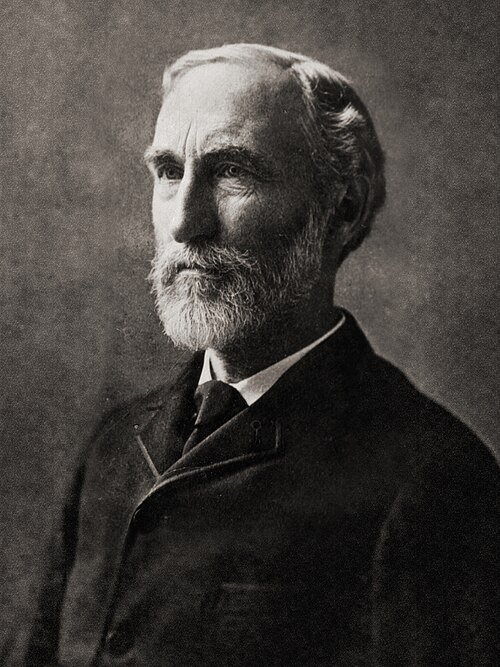
\includegraphics[width=\linewidth]{images/book3/gibbs.jpg}
\end{minipage}\hfill
\begin{minipage}[t]{0.76\linewidth}\vspace{0pt}
Josiah Willard Gibbs (1839--1903), professor of mathematical physics at
Yale, published between 1876 and 1878 \emph{On the Equilibrium of
Heterogeneous Substances}, some three hundred pages in the transactions of
a small academy, where the free energy, the chemical potential and the
phase rule of the next chapters all appear. Few chemists read it until it
was translated in the 1890s. (Photograph: public domain, Wikimedia
Commons.)
\end{minipage}
\end{history}

\section{Standard reaction Gibbs energies and temperature}

\begin{definition}[Ellingham approximation]\label{def:b2:reaction-free-energy:ellingham-approximation}
The \emph{Ellingham approximation}\index{Ellingham approximation} treats
$\Delta_r H^\circ$ and $\Delta_r S^\circ$ as independent of the temperature
over an interval containing no change of state. Then $\Delta_r G^\circ(T)
= \Delta_r H^\circ - T\Delta_r S^\circ$ is a straight line in $T$, of slope
$-\Delta_r S^\circ$.
\end{definition}

\begin{proposition}[Temperature derivatives]\label{prop:b2:reaction-free-energy:gibbs-helmholtz}
\[
  \frac{\dd\Delta_r G^\circ}{\dd T} = -\Delta_r S^\circ, \qquad
  \frac{\dd}{\dd T}\!\left(\frac{\Delta_r G^\circ}{T}\right) =
  -\frac{\Delta_r H^\circ}{T^2}\ \ \text{(Gibbs--Helmholtz)}, \qquad
  \frac{\dd\Delta_r S^\circ}{\dd T} = \frac{\Delta_r C^\circ_p}{T}.
\]
In particular the \omterm{def:b2:reaction-free-energy:ellingham-approximation}{Ellingham approximation} holds when $\Delta_r C^\circ_p$
is small.
\end{proposition}

\begin{proof}
With every species in its standard state, $G^\circ(T, \xi)$ has $(\partial
G^\circ/\partial T)_\xi = -S^\circ$ (\cref{prop:b2:reaction-free-energy:dG}).
By Schwarz's theorem,
\[
  \frac{\dd\Delta_r G^\circ}{\dd T} = \partial_\xi\partial_T G^\circ =
  -\partial_\xi S^\circ = -\Delta_r S^\circ .
\] Then $\frac{\dd}{\dd
T}(\Delta_r G^\circ/T) = \frac{-T\Delta_r S^\circ - \Delta_r G^\circ}{T^2} =
-\frac{\Delta_r H^\circ}{T^2}$. Finally, $\dd S^\circ_m = C^\circ_{p,m}\,\dd
T/T$ for each species (\cref{prop:b2:reaction-free-energy:absolute-entropy}),
and the same combination gives the last relation. If $\Delta_r C^\circ_p$ is
small, $\Delta_r H^\circ$ (Kirchhoff) and $\Delta_r S^\circ$ hardly change.
\end{proof}

\begin{definition}[Inversion temperature]\label{def:b2:reaction-free-energy:inversion-temperature}
When $\Delta_r H^\circ$ and $\Delta_r S^\circ$ have the same sign, the
\emph{inversion temperature}\index{inversion temperature} of the reaction is
the temperature where $\Delta_r G^\circ$ changes sign; in the \omterm{def:b2:reaction-free-energy:ellingham-approximation}{Ellingham
approximation}, $T_i = \Delta_r H^\circ/\Delta_r S^\circ$.
\end{definition}

\begin{omfigure}
\begin{tikzpicture}
\begin{axis}[
  width=0.72\linewidth, height=5.6cm, xmin=0, xmax=1600, ymin=0, ymax=260,
  axis x line=bottom, axis y line=left, xlabel={$T$ (K)}, ylabel={\unit{kJ/mol}},
  tick label style={font=\small}, label style={font=\small}, clip=false]
\addplot[omThm, very thick] table[x=T, y=DrH] {figdata/out/bachelor-2-thermo-data-calcite.dat};
\addplot[omDef, very thick] table[x=T, y=TDrS] {figdata/out/bachelor-2-thermo-data-calcite.dat};
\node[omThm, anchor=south west, font=\small] at (axis cs:60,180) {$\Delta_r H^\circ = 178.3$};
\node[omDef, anchor=west, font=\small] at (axis cs:1600,257) {$T\Delta_r S^\circ$};
\draw[dotted] (axis cs:1110,0) -- (axis cs:1110,178.3);
\node[anchor=south west, font=\small] at (axis cs:1120,8) {$T_i = \qty{1110}{K}$};
\node[font=\scriptsize, align=center] at (axis cs:600,140) {$\Delta_r G^\circ > 0$:\\ calcite stable};
\node[font=\scriptsize, align=center] at (axis cs:1470,206) {$\Delta_r G^\circ < 0$};
\end{axis}
\end{tikzpicture}

{\small The enthalpy and entropy terms of \ce{CaCO3(s) -> CaO(s) + CO2(g)}
in the \omterm{def:b2:reaction-free-energy:ellingham-approximation}{Ellingham approximation}. Below the \omterm{def:b2:reaction-free-energy:inversion-temperature}{inversion temperature} the
enthalpy cost wins and limestone is stable under \qty{1}{bar} of carbon
dioxide; above it the entropy term wins and limestone decomposes.}
% ledger: dfh:CaCO3_cr, dfh:CaO_cr, dfh:CO2, s0:CaCO3_cr, s0:CaO_cr, s0:CO2_g (computed in figdata/bachelor-2/thermo-data.py)
\end{omfigure}

\begin{omfigure}
\begin{tikzpicture}[font=\small]
  \draw[thick] (0,0) rectangle (8,4);
  \draw[thick] (4,0) -- (4,4) (0,2) -- (8,2);
  \node[above] at (2,4) {$\Delta_r H^\circ < 0$};
  \node[above] at (6,4) {$\Delta_r H^\circ > 0$};
  \node[left] at (0,3) {$\Delta_r S^\circ > 0$};
  \node[left] at (0,1) {$\Delta_r S^\circ < 0$};
  \node[align=center, omDef] at (2,3) {exergonic\\ at every $T$};
  \node[align=center, omProp] at (6,3) {exergonic\\ above $T_i$};
  \node[align=center, omProp] at (2,1) {exergonic\\ below $T_i$};
  \node[align=center, omThm] at (6,1) {endergonic\\ at every $T$};
\end{tikzpicture}

{\small The four cases of $\Delta_r G^\circ = \Delta_r H^\circ - T\Delta_r
S^\circ$ (\omterm{def:b2:reaction-free-energy:ellingham-approximation}{Ellingham approximation}). Combustions are in the upper left box;
the decomposition of limestone and the cold pack in the upper right; the
synthesis of ammonia in the lower left.}
\end{omfigure}

\begin{method}[A standard reaction Gibbs energy at temperature $T$]\label{met:b2:reaction-free-energy:delta-g-standard}
\begin{enumerate}
  \item From the tables at \qty{298.15}{K}, compute $\Delta_r H^\circ$ and
        $\Delta_r S^\circ$.
  \item Check that no species changes state between \qty{298}{K} and $T$;
        otherwise add the transition (enthalpy and entropy) or start from
        the new state.
  \item In the \omterm{def:b2:reaction-free-energy:ellingham-approximation}{Ellingham approximation}, $\Delta_r G^\circ(T) = \Delta_r H^\circ
        - T\Delta_r S^\circ$.
  \item Where $\Delta_r C^\circ_p$ is not small or the interval is long,
        use tabulated $\Delta_f G^\circ(T)$ directly.
\end{enumerate}
\end{method}

\begin{example}[Two tests of the approximation]\label{ex:b2:reaction-free-energy:tests}
For limestone, $\Delta_r C^\circ_p = 42.80 + 37.13 - 81.88 =
\qty{-2.0}{J/(K.mol)}$: the approximation is excellent, and $\Delta_r
G^\circ = 178.3 - T \times 0.1606$ gives $T_i = \qty{1110}{K}$. For ammonia,
$\Delta_r G^\circ(700) \approx -91.9 + 700 \times 0.1981 =
\qty{+46.8}{kJ/mol}$, while the tables give $2\Delta_f G^\circ(\ce{NH3}, 700) =
\qty{+54.4}{kJ/mol}$: here $\Delta_r C^\circ_p = \qty{-44}{J/(K.mol)}$ and
the error is \qty{8}{kJ/mol}, a factor of 4 on the equilibrium constant at
that temperature.
% ledger: cp:CaO_cr.298, cp:CO2_g.298, cp:CaCO3_cr.298, janafG:NH3.700 (computed in figdata/bachelor-2/thermo-data.py)
\end{example}

\section{Exercises}

\begin{exercise}[$\star$]\label{exo:b2:reaction-free-energy:1}
Predict the sign of $\Delta_r S^\circ$ for: (a) \ce{2H2(g) + O2(g) -> 2H2O(l)};
(b) \ce{CaCO3(s) -> CaO(s) + CO2(g)}; (c) \ce{N2O4(g) -> 2NO2(g)};
(d) \ce{Ag+(aq) + Cl-(aq) -> AgCl(s)}; (e) \ce{H2O(s) -> H2O(l)};
(f) \ce{H2(g) + Cl2(g) -> 2HCl(g)}.
\end{exercise}

\begin{exercise}[$\star$]\label{exo:b2:reaction-free-energy:2}
Compute $\Delta_r S^\circ$ and $\Delta_r G^\circ$ at \qty{298.15}{K} for the
synthesis of ammonia, \ce{N2(g) + 3H2(g) -> 2NH3(g)}, with $\Delta_r
H^\circ = \qty{-91.9}{kJ/mol}$ and the entropies of the chapter. Is it
\omterm{def:b2:reaction-free-energy:exergonic}{exergonic}?
\end{exercise}

\begin{exercise}[$\star$]\label{exo:b2:reaction-free-energy:3}
Compute $\Delta_r G^\circ(\qty{298.15}{K})$ of \ce{H2(g) + 1/2O2(g) ->
H2O(l)} from $\Delta_f H^\circ(\ce{H2O}, \text{l}) = \qty{-285.83}{kJ/mol}$
and the standard entropies \ce{H2(g)} 130.68, \ce{O2(g)} 205.15,
\ce{H2O(l)} \qty{69.95}{J/(K.mol)}. Why is this value the standard \omterm{def:b2:reaction-free-energy:gibbs-energy}{Gibbs
energy} of formation of liquid water?
% ledger: dfh:H2O-l, s0:H2_g, s0:O2_g, s0:H2O_l
\end{exercise}

\begin{exercise}[$\star$]\label{exo:b2:reaction-free-energy:4}
Use the figure of the entropy of zinc to read its \omterm{def:b2:reaction-free-energy:standard-entropy}{standard molar entropy} at
\qty{298}{K} and at \qty{1000}{K}, and its jumps at the melting and boiling
points. Deduce its enthalpies of fusion and of vaporisation.
\end{exercise}

\begin{exercise}[$\star\star$]\label{exo:b2:reaction-free-energy:5}
For \ce{H2O(l) -> H2O(g)} at \qty{298.15}{K}, compute $\Delta_r H^\circ$,
$\Delta_r S^\circ$ and $\Delta_r G^\circ$ from the tables of the chapter.
Explain why $\Delta_r S^\circ \neq \Delta_r H^\circ/T$ at \qty{298}{K}, what
the positive $\Delta_r G^\circ$ means, and estimate in the \omterm{def:b2:reaction-free-energy:ellingham-approximation}{Ellingham
approximation} the temperature at which liquid water and its vapour at
\qty{1}{bar} are in equilibrium. Compare with the boiling point.
\end{exercise}

\begin{exercise}[$\star\star$]\label{exo:b2:reaction-free-energy:6}
For \ce{N2O4(g) -> 2NO2(g)}, $\Delta_r H^\circ = \qty{57.1}{kJ/mol}$ and
$\Delta_r S^\circ = \qty{175.7}{J/(K.mol)}$. Compute the \omterm{def:b2:reaction-free-energy:inversion-temperature}{inversion
temperature}, and explain why a sealed tube of the brown gas \ce{NO2} pales
when it is cooled in ice.
\end{exercise}

\begin{exercise}[$\star\star$]\label{exo:b2:reaction-free-energy:7}
A reaction has $\Delta_r G^\circ = \qty{-12.0}{kJ/mol}$ at \qty{300}{K}
and $\qty{-4.0}{kJ/mol}$ at \qty{400}{K}. In the \omterm{def:b2:reaction-free-energy:ellingham-approximation}{Ellingham approximation},
find $\Delta_r H^\circ$ and $\Delta_r S^\circ$, and check the
Gibbs--Helmholtz relation.
\end{exercise}

\begin{exercise}[$\star\star$]\label{exo:b2:reaction-free-energy:8}
Compute $\Delta_r G^\circ$ of the formation of methane, \ce{C(s) + 2H2(g) ->
CH4(g)}, at \qty{298.15}{K}, from $\Delta_f H^\circ = \qty{-74.87}{kJ/mol}$
and the entropies \ce{C} (graphite) 5.74, \ce{H2} 130.68, \ce{CH4}
\qty{186.25}{J/(K.mol)}. Above which temperature does methane become
unstable with respect to its elements under the standard pressure?
% ledger: dfh:CH4_g, s0:C_gr, s0:H2_g, s0:CH4_g
\end{exercise}

\begin{exercise}[$\star\star$]\label{exo:b2:reaction-free-energy:9}
A haloalkane reacts with a base by substitution or by elimination. Write
both reactions for 2-bromopropane and hydroxide. With $\Delta_r
H^\circ(\text{elimination}) - \Delta_r H^\circ(\text{substitution}) =
\qty{+40}{kJ/mol}$ and $\Delta_r S^\circ(\text{elimination}) - \Delta_r
S^\circ(\text{substitution}) = \qty{+90}{J/(K.mol)}$ (orders of magnitude),
find above which temperature the elimination becomes the more \omterm{def:b2:reaction-free-energy:exergonic}{exergonic} of
the two, and explain the role of the number of molecules.
\end{exercise}

\begin{exercise}[$\star\star\star$]\label{exo:b2:reaction-free-energy:10}
Crystalline carbon monoxide does not reach zero entropy at \qty{0}{K}: each
molecule can sit as CO or OC almost at random, the two orientations having
nearly the same energy. Admitting Boltzmann's formula $S = k_B\ln W$, where
$W$ is the number of arrangements (counted in the Year 3 volume), compute
the residual molar entropy. Why does the third law not apply to this
crystal?
\end{exercise}

\begin{exercise}[$\star\star\star$]\label{exo:b2:reaction-free-energy:11}
Show that if $\Delta_r C^\circ_p$ is a constant $c$,
$\Delta_r S^\circ(T) = \Delta_r S^\circ(T_0) + c\ln(T/T_0)$ and
$\Delta_r G^\circ(T) = \Delta_r H^\circ(T_0) - T\Delta_r S^\circ(T_0) +
c\,[T - T_0 - T\ln(T/T_0)]$. Apply it to limestone ($c =
\qty{-2.0}{J/(K.mol)}$) at \qty{1100}{K}, and measure the error of the
\omterm{def:b2:reaction-free-energy:ellingham-approximation}{Ellingham approximation}.
\end{exercise}

\begin{exercise}[$\star\star\star$]\label{exo:b2:reaction-free-energy:12}
Titanium is made from its oxide, rutile, through its chloride. (a) Compute
$\Delta_r H^\circ$ and $\Delta_r S^\circ$ at \qty{298}{K} of \ce{TiO2(s) +
2Cl2(g) -> TiCl4(g) + O2(g)}, with \ce{TiO2} ($-944.0$ \unit{kJ/mol},
\qty{50.62}{J/(K.mol)}) and \ce{TiCl4(g)} ($-763.2$, 353.2), and its
$\Delta_r G^\circ$ at \qty{1000}{K} in the \omterm{def:b2:reaction-free-energy:ellingham-approximation}{Ellingham approximation}.
(b) Carbon is added: \ce{C(s) + O2(g) -> CO2(g)}, $\Delta_r H^\circ =
\qty{-393.5}{kJ/mol}$, $\Delta_r S^\circ = \qty{+2.9}{J/(K.mol)}$. Compute
$\Delta_r G^\circ(\qty{1000}{K})$ of the sum of the two reactions and
explain how the second drives the first.
% ledger: dfh:TiO2_cr, s0:TiO2_cr, dfh:TiCl4_g, s0:TiCl4_g, s0:Cl2_g, s0:O2_g, s0:C_gr, s0:CO2_g
\end{exercise}

\section{Problem: The Lime Kiln}

\begin{problem}[{Weekend problem --- the entropy and enthalpy of a
decomposition, its Gibbs energy against temperature, the evolution
criterion in a kiln, and the energy and carbon dioxide of a tonne of
lime}]
\label{pb:b2:reaction-free-energy:1}
Lime, \ce{CaO}, is made by heating limestone, \ce{CaCO3}, in a kiln. Data at
\qty{298.15}{K}: $\Delta_f H^\circ$ (\unit{kJ/mol}) \ce{CaCO3(s)}
$-1206.92$, \ce{CaO(s)} $-635.09$, \ce{CO2(g)} $-393.51$; $S^\circ_m$
(\unit{J/(K.mol)}) 92.9, 39.75, 213.79; $C^\circ_{p,m}$ (\unit{J/(K.mol)})
81.88, 42.80, 37.13. Molar masses: \ce{CaO} \qty{56.08}{g/mol}, \ce{CO2}
\qty{44.01}{g/mol}, \ce{CH4} \qty{16.04}{g/mol}; combustion of methane,
water as vapour, $\Delta_r H^\circ = \qty{-802.3}{kJ/mol}$.
% ledger: dfh:CaCO3_cr, dfh:CaO_cr, dfh:CO2, s0:CaCO3_cr, s0:CaO_cr, s0:CO2_g, cp:CaCO3_cr.298, cp:CaO_cr.298, cp:CO2_g.298

\medskip
\noindent\textbf{Part I --- At room temperature.}
\begin{enumerate}
  \item Write the decomposition of limestone.
  \item Compute $\Delta_r H^\circ(\qty{298}{K})$. Is the reaction \omterm{def:b2:reaction-enthalpy:exothermic}{exothermic}?
  \item Compute $\Delta_r S^\circ(\qty{298}{K})$ and explain its sign.
  \item Compute $\Delta_r G^\circ(\qty{298}{K})$.
  \item Is limestone stable at room temperature under \qty{1}{bar} of
        carbon dioxide? Why do limestone cliffs last?
  \item Compute $\Delta_r C^\circ_p$, and say what it implies for the
        temperature dependence of $\Delta_r H^\circ$ and $\Delta_r S^\circ$.
\end{enumerate}

\medskip
\noindent\textbf{Part II --- Heating.}
\begin{enumerate}[resume]
  \item Write $\Delta_r G^\circ(T)$ in the \omterm{def:b2:reaction-free-energy:ellingham-approximation}{Ellingham approximation}.
  \item Compute it at \qty{1000}{K} and at \qty{1300}{K}.
  \item Compute the \omterm{def:b2:reaction-free-energy:inversion-temperature}{inversion temperature} $T_i$.
  \item Check the Gibbs--Helmholtz relation on this expression.
  \item Estimate, with the formula of \cref{exo:b2:reaction-free-energy:11},
        the change of $\Delta_r G^\circ$ at $T_i$ caused by
        $\Delta_r C^\circ_p$, and the resulting shift of $T_i$.
\end{enumerate}

\medskip
\noindent\textbf{Part III --- The kiln.}
In this part the carbon dioxide above the solids is at \qty{1}{bar}, so
that $\Delta_r G = \Delta_r G^\circ$.
\begin{enumerate}[resume]
  \item What does the evolution criterion say at \qty{1000}{K}? And at
        \qty{1300}{K}?
  \item What happens to a mixture of lime and carbon dioxide at
        \qty{1}{bar} cooled below $T_i$?
  \item How much entropy is created per mole of limestone decomposed at
        \qty{1300}{K}?
  \item Kilns are swept by the combustion gases, poorer in carbon dioxide.
        Guess, before the next chapter, whether this helps the
        decomposition.
\end{enumerate}

\medskip
\noindent\textbf{Part IV --- A tonne of lime.}
\begin{enumerate}[resume]
  \item Compute the amount of lime in one tonne.
  \item Compute the heat absorbed by the reaction per tonne of lime
        (take $\Delta_r H^\circ$ as constant).
  \item Compute the mass of carbon dioxide released by the limestone per
        tonne of lime.
  \item The heat comes from burning methane with a useful efficiency of
        50\,\%. Compute the mass of methane burnt per tonne of lime.
  \item Compute the carbon dioxide from this methane.
  \item Compute the total carbon dioxide per tonne of lime, and the share
        due to the limestone itself.
  \item Why can a cleaner fuel reduce only part of these emissions?
  \item State the temperature above which limestone decomposes under
        \qty{1}{bar} of carbon dioxide.
\end{enumerate}
\end{problem}
